\subsection{Mediator}
\label{mediator}

\textbf{Scopo}: Comportamentale \\
\textbf{Raggio d'azione}: Oggetti

\paragraph{Definizione} Il pattern permette di definire un oggetto che incapsula il modo in cui un insieme di oggetti interagisce. Mediator promuove un accoppiamento debole impedendo agli oggetti di fare riferimento esplicito gli uni agli altri e consente di variare la loro interazione in modo indipendente.

\paragraph{Motivazione} La progettazione orientata agli oggetti incoraggia la distribuzione del comportamento tra oggetti, ma tale distribuzione può risultare in una struttura di oggetti con molte connessioni tra di essi, dove nel caso peggiore ogni oggetto finisce per conoscere ogni altro oggetto.

\begin{figure}[H]
    \centering
    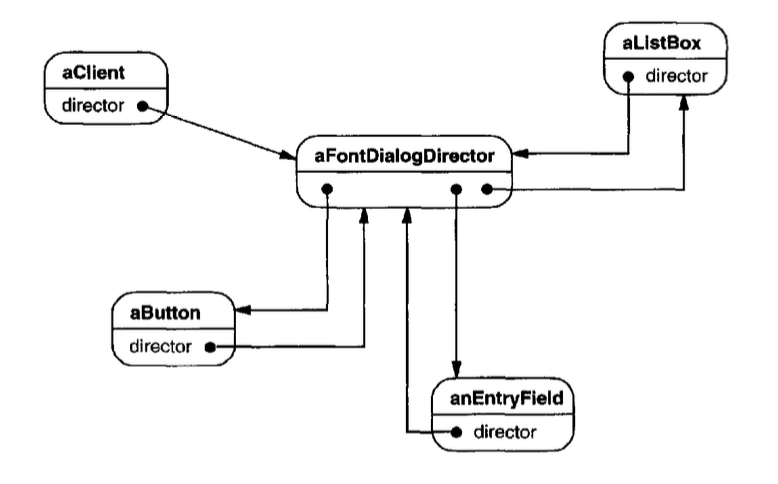
\includegraphics[width=0.5\linewidth]{assets/pattern/mediator/mediator-esempio-object.png}
\end{figure}

Anche se partizionare un sistema in molti oggetti generalmente migliora la riusabilità, le interconnessioni proliferanti tendono a ridurla nuovamente, rendendo meno probabile che un oggetto possa funzionare senza il supporto di altri e facendo sì che il sistema agisca come se fosse monolitico.

\begin{figure}[H]
    \centering
    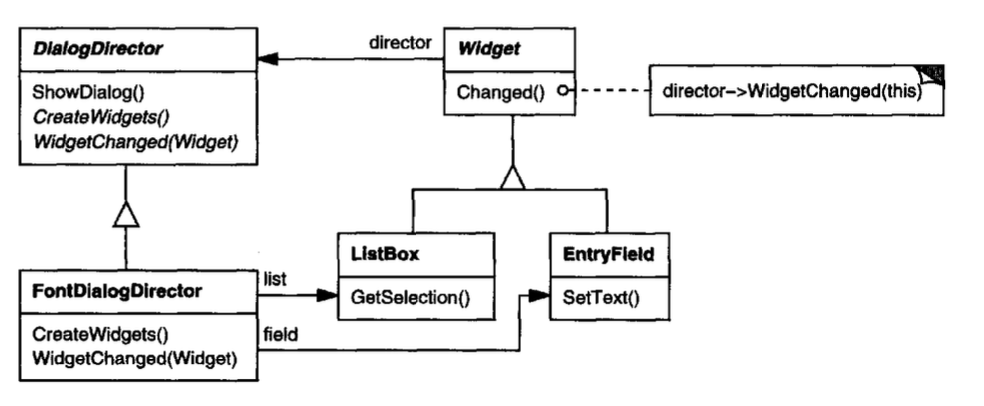
\includegraphics[width=0.75\linewidth]{assets/pattern/mediator/mediator-esempio-class.png}
\end{figure}

Inoltre può essere difficile cambiare il comportamento del sistema in modo significativo, poiché il comportamento è distribuito tra molti oggetti, e di conseguenza potresti essere costretto a definire molte sottoclassi per personalizzare il comportamento del sistema. Come esempio, considera l'implementazione di finestre di dialogo in un'interfaccia grafica utente, dove spesso ci sono dipendenze tra i widget nella finestra di dialogo: un pulsante viene disabilitato quando un certo campo di inserimento è vuoto, selezionare una voce in una lista potrebbe cambiare i contenuti di un campo di inserimento, e viceversa digitare testo nel campo potrebbe automaticamente selezionare una o più voci corrispondenti nella lista.

\begin{figure}[H]
    \centering
    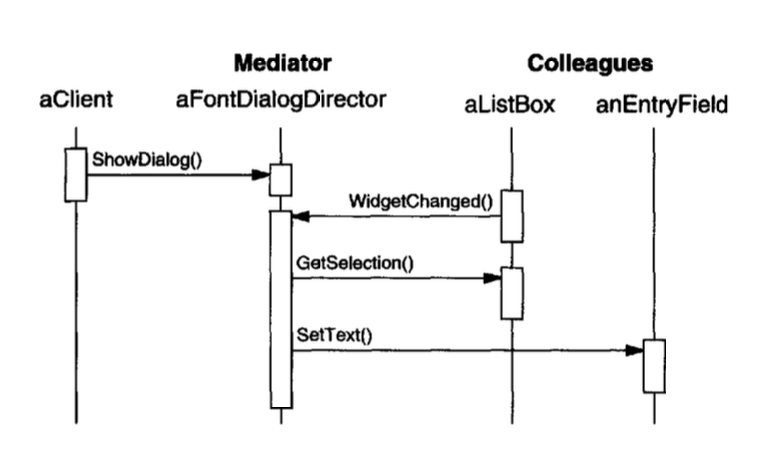
\includegraphics[width=0.75\linewidth]{assets/pattern/mediator/mediator-esempio-sequence.png}
\end{figure}

Diverse finestre di dialogo avranno diverse dipendenze tra widget, quindi anche se le finestre mostrano gli stessi tipi di widget, non possono semplicemente riusare classi widget standard ma devono essere personalizzate per riflettere dipendenze specifiche della finestra, e personalizzarle individualmente tramite sottoclassi sarebbe tedioso poiché molte classi sono coinvolte. Puoi evitare questi problemi incapsulando il comportamento collettivo in un oggetto mediatore separato che è responsabile del controllo e coordinamento delle interazioni di un gruppo di oggetti, servendo come intermediario che impedisce agli oggetti nel gruppo di riferirsi l'uno all'altro esplicitamente, dove gli oggetti conoscono solo il mediatore, riducendo così il numero di interconnessioni.

\paragraph{Applicabilità} È consigliabile utilizzare il pattern Mediator quando:
\begin{itemize}
    \item Gli oggetti comunicano in modi ben definiti ma complessi. Le interdipendenze che ne derivano sono destrutturate e difficili da comprendere.
    \item Riutilizzare un oggetto è difficile perché esso fa riferimento e comunica con molti altri oggetti.
    \item Un comportamento distribuito tra diverse classi dovrebbe essere personalizzabile senza ricorrere a un numero eccessivo di sottoclassi.
\end{itemize}

\begin{figure}[H]
    \centering
    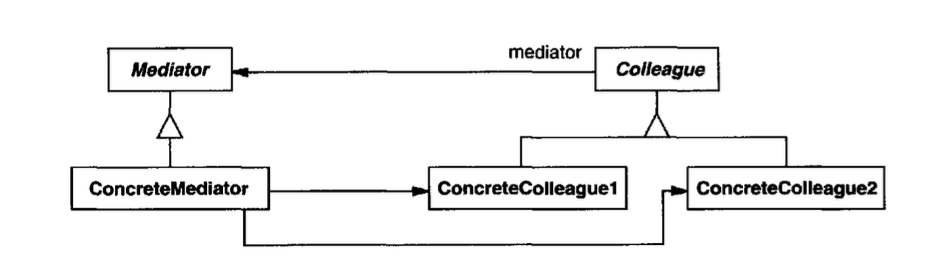
\includegraphics[width=0.75\linewidth]{assets/pattern/mediator/mediator-struttura.png}
    \caption{Class Diagram del pattern Mediator}
\end{figure}

\newpage

\paragraph{Struttura}
\begin{itemize}
    \item \textbf{Mediator}: definisce un’interfaccia che espone i metodi che abilitano la comunicazione tra i componenti in relazione o agisce come punto centrale per la gestione delle interazioni tra i vari partecipanti. Il Mediatore conosce e mantiene i riferimenti agli oggetti dei partecipanti e facilita la loro comunicazione. Gestisce le dipendenze e incapsula il comportamento.
    \item \textbf{ConcreteMediator}: implementa l’interfaccia Mediator e, nel definire i metodi dell’interfaccia, realizza uno specifico comportamento di cooperazione tra i componenti. Gestisce effettivamente la comunicazione tra i partecipanti, implementando i metodi definiti nell'interfaccia del Mediatore. Essa conosce i partecipanti e regola il flusso delle comunicazioni tra di essi.
    \item \textbf{Colleague}: definisce l’interfaccia che rappresenta un componente del sistema che deve comunicare tramite il Mediatore. Ogni Colleague conosce solo il Mediatore e non ha una conoscenza diretta degli altri Colleague. Essi inviano e ricevono messaggi tramite il Mediatore.
    \item \textbf{ConcreteColleague}: classe concreta che implementa l'interfaccia dei Colleague. Ogni ConcreteColleague è un componente specifico del sistema che deve comunicare con gli altri Colleague tramite il Mediatore.
\end{itemize}

Il pattern mediator permette di limitare la sottoclasse del comportamento, separare i colleghi, semplificare i protocolli degli oggetti, facilitare l’aggiunta di nuovi componenti, astrarre la cooperazione tra oggetti, favorire il riutilizzo dei Mediator e centralizzare il controllo delle interazioni.

\paragraph{Conseguenze} Il pattern Mediator consente quindi di:
\begin{itemize}
    \item Limitare il \textit{subclassing};
    \item Disaccoppiare gli oggetti Colleague;
    \item Semplificare i protocolli degli oggetti;
    \item Astrarre il modo in cui gli oggetti cooperano;
    \item Centralizzare il controllo;
\end{itemize}

\paragraph{Pattern correlati}
\begin{itemize}
    \item \textbf{Observer} (\ref{observer})
    \item \textbf{Facade} (\ref{facade})
    \item \textbf{Command} (\ref{command})
    \item \textbf{Chain of Responsibility} (\ref{chain-of-responsability})
    \item \textbf{Strategy} (\ref{strategy})
\end{itemize}


\paragraph{Nota} È bene notare che la POO incoraggia la distribuzione di comportamento tra gli oggetti, portando ad una struttura con molte connesioni tra oggetti. Le molte interconnessioni rendono meno probabile che un oggetto possa funzionare senza il supporto di altri.

\newpage